The proposed solution of the SSDTA can be used in a wide range of optimization procedures. One of them is reliability optimization that we discuss in this section. We perform a temperature-aware task mapping and scheduling in order to address the thermal cycling ageing effect while keeping the energy consumption at an appropriate level. Both mapping and scheduling are based on a genetic algorithm \cite{schmitz2004}.

\subsection{Application Model} \label{sec:application-model}
The overall structure of the periodic application is modeled as a task graph $G = (V, \: E, \: \period)$ where $V$ is a set of $N_t$ tasks (vertices of the graph), $E$ is a set of data dependencies between tasks (edges), and $\period$ is the period of the application, which we assume to be equal to the deadline. Each pair of a task $v_i \in V$ and processing element $\pi_j \in \Pi$ is characterized by a tuple $(N_{clock \: ij}, C_{eff \; ij})$, where $N_{clock \: ij}$ is the number of clock cycles and $C_{eff \; ij}$ is the effective switched capacitance. These parameters along with the architecture (\secref{sec:architecture-model}) and power (\secref{sec:power-model}) models determine the execution time of the task and processor load, respectively.

\subsection{Temperature-Aware Reliability Model} \label{sec:reliability-model}
We address temperature-driven failure mechanisms with the reliability model presented in \cite{huang2009}, \cite{xiang2010}. The model is based on the assumption that the time to failure $\mathcal{T}$ has a Weibull distribution:
\begin{align}
  & \mathcal{T} \sim Weibull(\eta, \beta) \nonumber \\
  & \expectation{\mathcal{T}} = \eta \; \Gamma(1 + \frac{1}{\beta}) \label{eq:general-mttf}
\end{align}
where $\eta$ and $\beta$ are the scaling and shape parameters of the distribution, respectively, $\Gamma$ is the gamma function. The expectation given by \equref{eq:general-mttf} is the mean time to failure (MTTF) that we denote by $\theta = \expectation{\mathcal{T}}$.

The shape parameter $\beta$ is found to be independent on the temperature variation \cite{chang2006}, which, however, is not the case with the scaling parameter $\eta$. Therefore, the distribution varies with the temperature. We can split the overall period of the application $\period$ into $N_m$ time intervals $\Delta t_i$, so that during each time interval $\Delta t_i$ the corresponding $\eta_i$ is a constant:
\begin{equation} \label{eq:eta-one}
  \eta_i = \frac{\theta_i}{\Gamma(1 + \frac{1}{\beta})}
\end{equation}
where $\theta_i$ is the MTTF in the $i$th time interval as if we had the failure distribution of this interval all the time. For now the values $\theta_i$ are unknown and depend on the particular failure mechanism. As it is shown in \cite{xiang2010}, the reliability function $R(t)$, i.e., the probability of survival until an arbitrary time $t \geq 0$, can be approximated as the following:
\[
  R(t) = e^{-(\frac{t}{\period} \sum_{i=0}^{N_m - 1} \frac{\Delta t_i}{\eta_i})^\beta}
\]
The formula keeps the form of the Weibull distribution with the scaling parameter equal to:
\begin{equation} \label{eq:eta-many}
  \eta = \frac{\period}{\sum_{i=0}^{N_m - 1} \frac{\Delta t_i}{\eta_i}}
\end{equation}
Consequently, the MTTF with respect to the whole application period can be obtained by combining \equref{eq:general-mttf}, \equref{eq:eta-one}, and \equref{eq:eta-many}.

As mentioned previously, in order to compute the MTTF, we need to consider the particular failure mechanism and determine the values $\theta_i$ needed in \equref{eq:eta-one}. In this paper, our focus is on the thermal cycling (TC) fatigue, which is directly connected to the temperature variations. According to this model, the parameters affecting reliability are the amplitude and number of thermal cycles as well as the maximal temperature. A thermal cycle is a time interval in which the temperature starts from a certain value and, after reaching an extremum, returns to the starting point. We follow the approach given in \cite{xiang2010} where the rainflow counting method is employed to identify thermal cycles in the temperature curve. Assuming this concrete failure model the duration $\Delta t_i$, during which the corresponding scaling parameter $\eta_i$ is constant \equref{eq:eta-one}, is exactly a thermal cycle.

When the system is exposed to identical thermal cycles, the number of such cycles to failure can be estimated using a modified version of the well-known Coffin-Manson equation with the Arrhenius term \cite{xiang2010}, \cite{jedec2010}, \cite{ciappa2003}:
\begin{equation} \label{eq:cycles-to-failure}
  N_c = A (\Delta T - \Delta T_0)^{-b} e^{\frac{E_a}{k T_{max}}}
\end{equation}
where $A$ is an empirically determined constant, $\Delta T$ is the thermal cycle excursion (the distance between the minimal and maximal temperatures), $\Delta T_0$ is the portion of the temperature range in the elastic region which does not cause damage, $b$ is the Coffin-Manson exponent which is also empirically determined, $E_{a}$ is the activation energy, $k$ is the Boltzmann constant, and $T_{max}$ is the maximal temperature during the thermal cycle. The system undergoes a number of different thermal cycles each with its own duration $\Delta t_i$ over the application period and each cycle causes its own damage. Therefore, having $N_m$ thermal cycles characterized by the number of cycles to failure $N_{c\:i}$ and duration $\Delta t_i$, we can compute $\theta_i$:
\begin{equation} \label{eq:mttf-cycle}
  \theta_i = N_{c \: i} \; \Delta t_i
\end{equation}
Taking equations \eqref{eq:general-mttf}, \eqref{eq:eta-one}, \eqref{eq:eta-many}, and \eqref{eq:mttf-cycle} together, we obtain the following expression to estimate the MTTF of one component in the system:
\begin{align} \label{eq:one-mttf}
  \theta = \frac{\period}{\sum_{i=0}^{N_m - 1} \frac{1}{N_{c \: i}}}
\end{align}

It can be observed that the final equation includes the sum over $N_{c \: i}$ defined by \equref{eq:cycles-to-failure}. The computation requires the identification of the thermal cycles with their amplitudes and maximal temperatures. All the prerequisites are captured by the SSDTP, which is needed as an input to the reliability optimization.

\subsection{Motivational Example} \label{sec:motivation}
Consider an application with six tasks, denoted ``T0''--``T5'', and a heterogeneous architecture with two cores, labeled ``PE0'' and ``PE1''. The task graph of the application is given in \figref{fig:task-graph} along with the execution times for both cores. The period of the application is 0.06 seconds. A first alternative mapping and schedule, and the resulting SSDTP are shown at the top of \figref{fig:motivation} (where the hight of a task represents its relative dynamic power consumption). It can be observed that initially PE0 is experiencing three thermal cycles. If we change the mapping of T5 and move it to PE1, we achieve two thermal cycles of PE0 instead of three. Finally, if we vary the schedule as well and change the order of T1 and T3, the number of cycles of PE0 becomes one. Using the reliability model from \secref{sec:reliability-model}, we observe improvements in the MTTF of 44.69\% and 54.53\%, respectively, relative to the initial configuration.
\begin{figure}
  \centering
  \subfloat[The task graph.]{
    \label{fig:task-graph}
    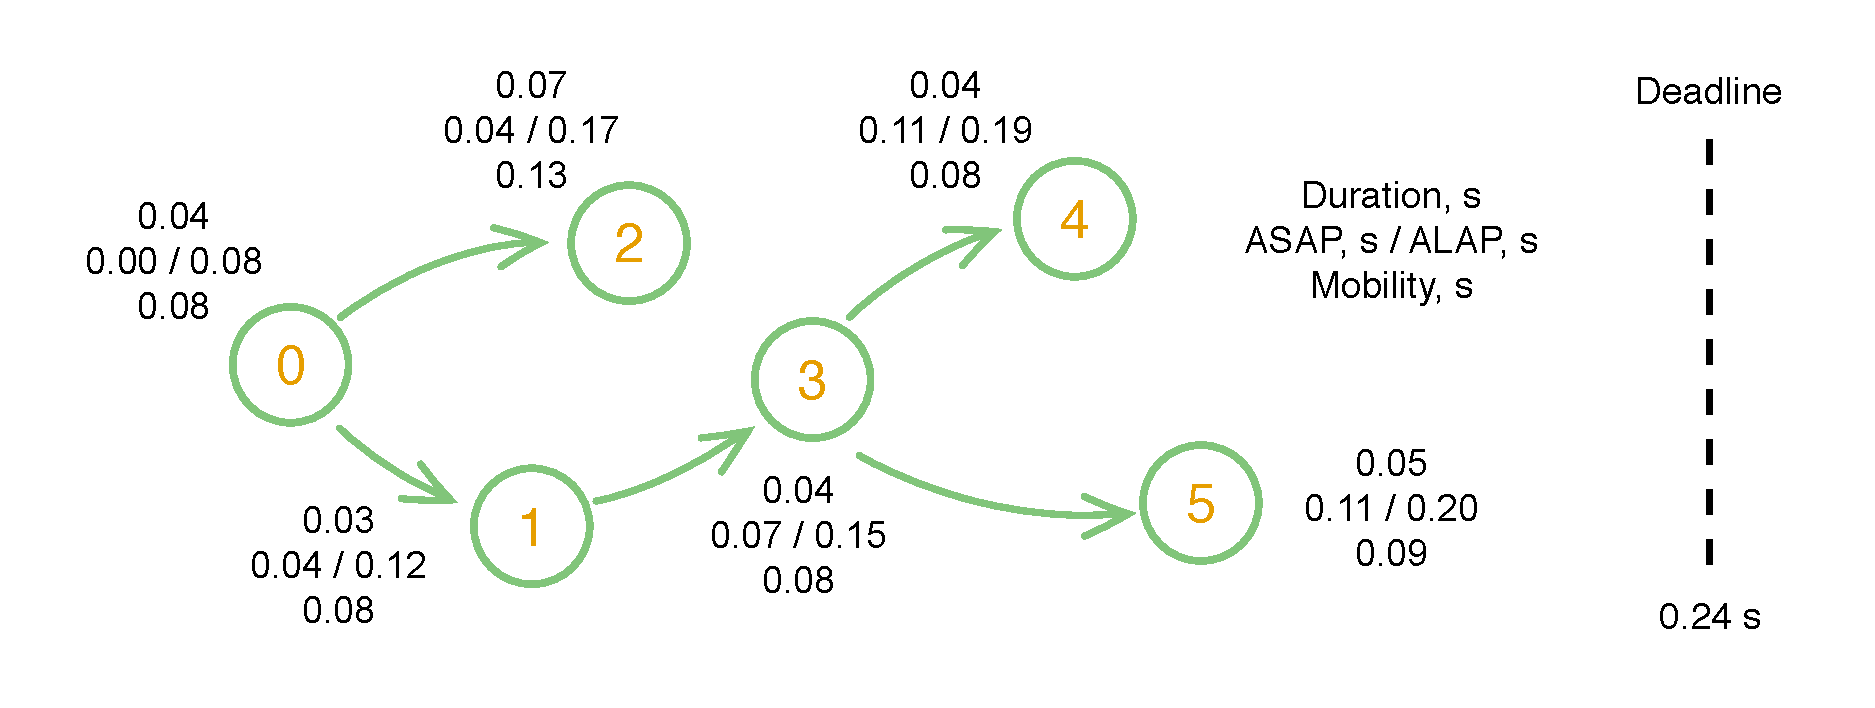
\includegraphics[width=0.8\linewidth]{assets/task-graph.pdf}
  }
  \vspace{-15pt}

  \subfloat[Alternative mappings and schedules.]{
    \label{fig:motivation}
    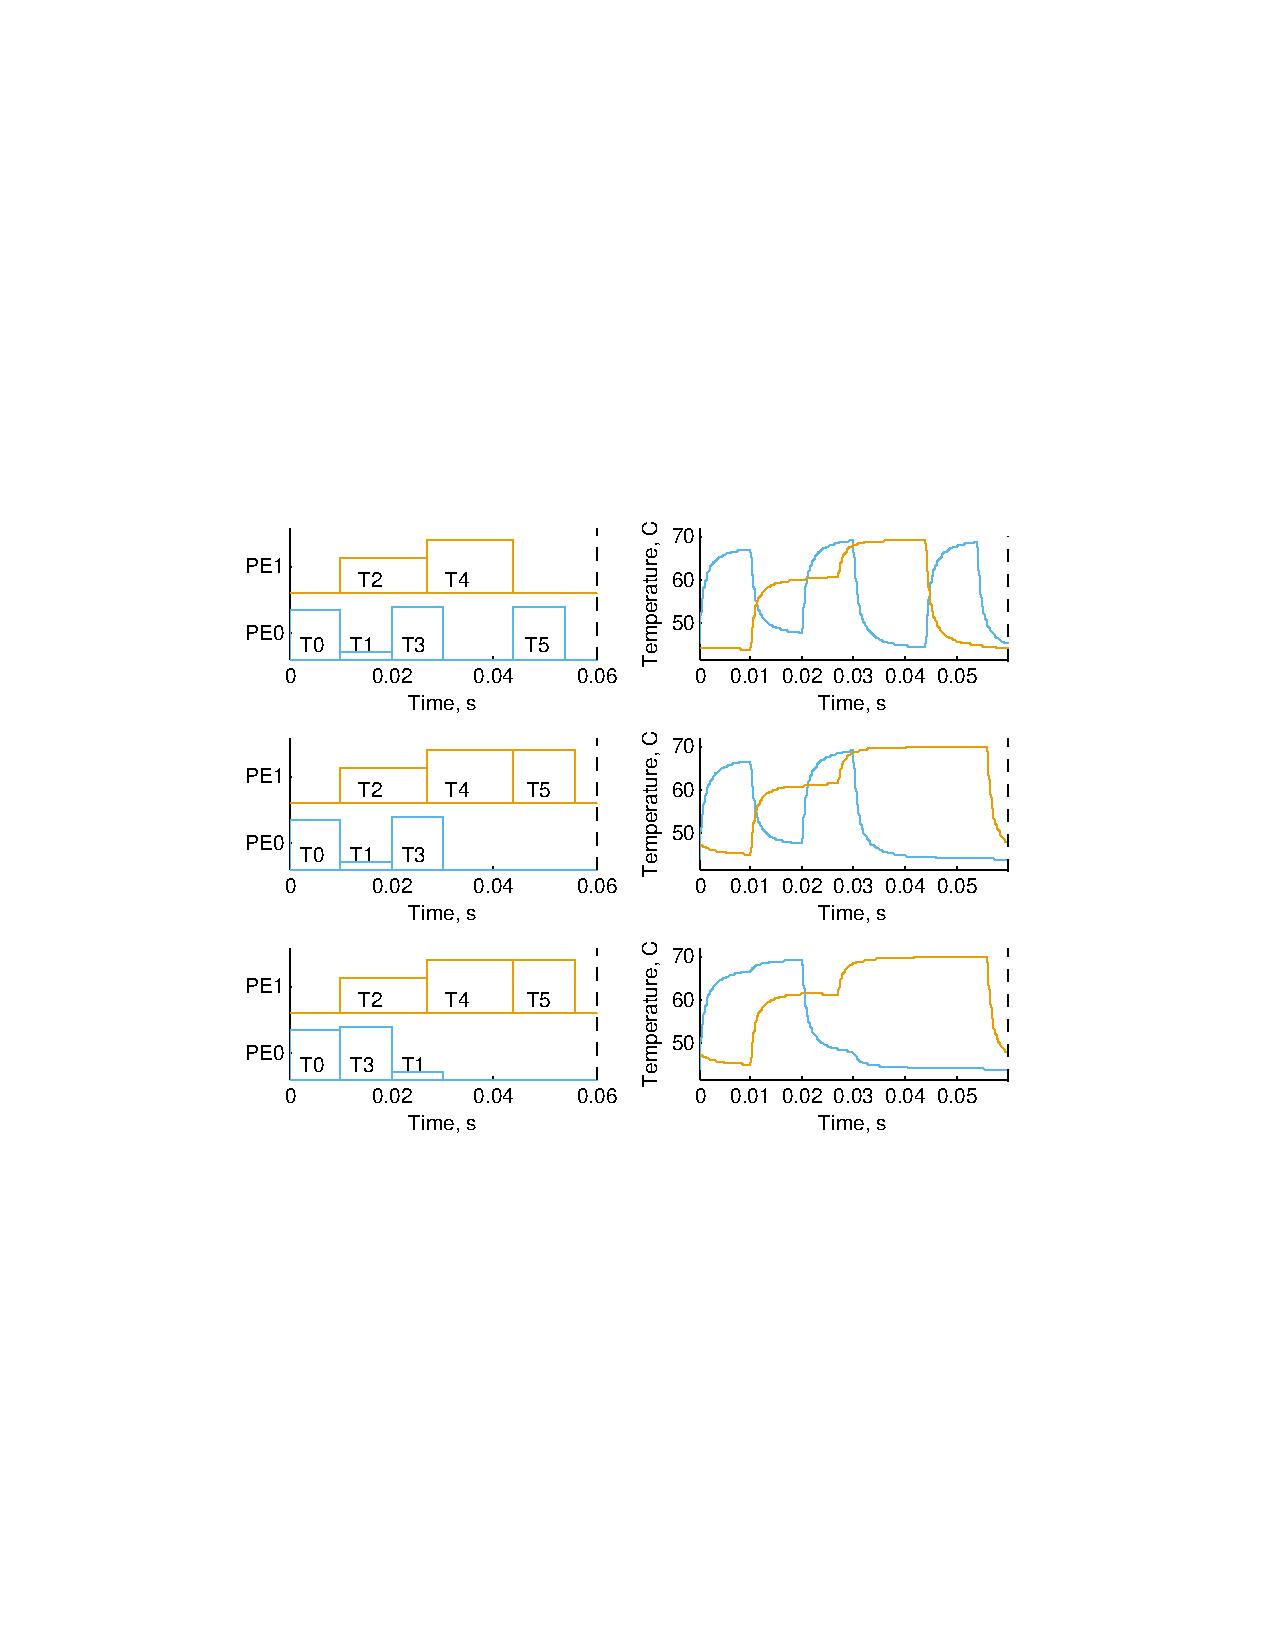
\includegraphics[width=0.8\linewidth]{assets/motivation.pdf}
  }
  \vspace{5pt}
  \caption{Motivational example.}
  \vspace{15pt}
\end{figure}


\subsection{Problem Formulation and Optimization} \label{sec:reliability-problem}
The objective of the optimization procedure is to prolong the lifetime of the system by varying the mapping and scheduling of the application being executed. The problem formulation is the following.

Given:

\begin{itemize}
  \item A multiprocessor system $\Pi$ (\secref{sec:architecture-model}).
  \item A periodic application $G$ (\secref{sec:application-model}).
  \item The floorplan of the chip at the desired level of details (\secref{sec:thermal-model}), configuration of the thermal package, and thermal parameters (\secref{sec:problem}).
  \item The parameters of the reliability model (\secref{sec:reliability-model}), i.e., the constants $A$, $\Delta T_0$, $b$, $E_a$ (see \equref{eq:cycles-to-failure}).
\end{itemize}

Maximize:
\begin{align}
  & F = \min_{i = 0}^{N_p - 1} \theta_i \label{eq:fitness-function} \\
  & s.t. \nonumber \\
  & Duration(G) \leq \period \label{eq:deadline} \\
  & T_{ij} \leq T_{max}, \; i = 0 \cdots N_s, j = 0 \dots N_p \label{eq:t-max}
\end{align}
where $\theta_i$ is the MTTF of the $i$th processing element given by \equref{eq:one-mttf}, $Duration(G)$ denotes the execution time of the application mapped and scheduled onto the platform, $\period$ is the period of the application, and $T_{ij}$ are temperature values in the SSDTP. \equref{eq:deadline} imposes the first constrain on the optimization where the application is to meet its deadline, which we assume to be equal to the period. \equref{eq:t-max} enforses the second constrain on the maximal temperature in the temperature profile $\mathbb{T} = \{ T_{ij} \}$.

The optimization procedure is held by a genetic algorithm (GA) \cite{schmitz2004} with the fitness function given by \equref{eq:fitness-function}. Each chromosome is a vector of $2 \times N_t$ elements, where the first half encodes priorities of the tasks and the second represents a mapping. The population contains $4 \times N_t$ individuals that are initialized partially randomly and partially based on the mobility of the tasks \cite{schmitz2004}. Each generation, a number of individuals, called parents, are chosen for breeding by the tournament selection with the number of competitors proportional to the population size. The parents undergo the 2-point crossover with $0.8$ probability and uniform mutation with $0.05$ probability. The evolution mechanism follows the elitism model where the best individual always survives. The stopping condition is an absence of improvement within $200$ successive generations.

The fitness of a chromosome, \equref{eq:fitness-function}, is evaluated in a number of steps. First, the decoded priorities and mapping are given to a list scheduler that produces schedules for each of the cores. If the schedules do not respect the deadline of the application, the solution is penalized proportionally to the delay and is not further evaluated; otherwise, based on the parameters of the architecture and tasks, a power profile is obtained and the corresponding SSDTP is computed by the CE method. If the SSDTP violates the temparature constrain given by \equref{eq:t-max}, the solution is penalized proportionaly to the amount of violation and not further processed; otherwise, the MTTF of each core is estimated according to \equref{eq:one-mttf} and the fitness function $F$ is computed.

